
%%%%%%%%%%%%%%%%%%%%%%%%%%%%%%%%%%%%%%%%%%%%%%%%%%%%%%%%%%%%%%%%%%%%%
%% This is a (brief) model paper using the achemso class
%% The document class accepts keyval options, which should include
%% the target journal and optionally the manuscript type.
%%%%%%%%%%%%%%%%%%%%%%%%%%%%%%%%%%%%%%%%%%%%%%%%%%%%%%%%%%%%%%%%%%%%%
\documentclass[journal=ancac3,manuscript=article]{achemso}

%%%%%%%%%%%%%%%%%%%%%%%%%%%%%%%%%%%%%%%%%%%%%%%%%%%%%%%%%%%%%%%%%%%%%
%% Place any additional packages needed here.  Only include packages
%% which are essential, to avoid problems later. Do NOT use any
%% packages which require e-TeX (for example etoolbox): the e-TeX
%% extensions are not currently available on the ACS conversion
%% servers.
%%%%%%%%%%%%%%%%%%%%%%%%%%%%%%%%%%%%%%%%%%%%%%%%%%%%%%%%%%%%%%%%%%%%%
\usepackage[version=3]{mhchem} % Formula subscripts using \ce{}
\usepackage[T1]{fontenc}       % Use modern font encodings
\usepackage{graphicx}
%%%%%%%%%%%%%%%%%%%%%%%%%%%%%%%%%%%%%%%%%%%%%%%%%%%%%%%%%%%%%%%%%%%%%
%% If issues arise when submitting your manuscript, you may want to
%% un-comment the next line.  This provides information on the
%% version of every file you have used.
%%%%%%%%%%%%%%%%%%%%%%%%%%%%%%%%%%%%%%%%%%%%%%%%%%%%%%%%%%%%%%%%%%%%%
%%\listfiles

%%%%%%%%%%%%%%%%%%%%%%%%%%%%%%%%%%%%%%%%%%%%%%%%%%%%%%%%%%%%%%%%%%%%%
%% Place any additional macros here.  Please use \newcommand* where
%% possible, and avoid layout-changing macros (which are not used
%% when typesetting).
%%%%%%%%%%%%%%%%%%%%%%%%%%%%%%%%%%%%%%%%%%%%%%%%%%%%%%%%%%%%%%%%%%%%%
\newcommand*\mycommand[1]{\texttt{\emph{#1}}}

%%%%%%%%%%%%%%%%%%%%%%%%%%%%%%%%%%%%%%%%%%%%%%%%%%%%%%%%%%%%%%%%%%%%%
%% Meta-data block
%% ---------------
%% Each author should be given as a separate \author command.
%%
%% Corresponding authors should have an e-mail given after the author
%% name as an \email command. Phone and fax numbers can be given
%% using \phone and \fax, respectively; this information is optional.
%%
%% The affiliation of authors is given after the authors; each
%% \affiliation command applies to all preceding authors not already
%% assigned an affiliation.
%%
%% The affiliation takes an option argument for the short name.  This
%% will typically be something like "University of Somewhere".
%%
%% The \altaffiliation macro should be used for new address, etc.
%% On the other hand, \alsoaffiliation is used on a per author basis
%% when authors are associated with multiple institutions.
%%%%%%%%%%%%%%%%%%%%%%%%%%%%%%%%%%%%%%%%%%%%%%%%%%%%%%%%%%%%%%%%%%%%%
\author{Nicholas P. Montoni}
\author{Steven C. Quillin}
\author{Charles Cherqui}
\author{David J. Masiello}
\email{masiello@chem.washington.edu}
\phone{}
\fax{}
\affiliation[University of Washington]
{Department of Chemistry, University of Washington, Seattle, WA}

%%%%%%%%%%%%%%%%%%%%%%%%%%%%%%%%%%%%%%%%%%%%%%%%%%%%%%%%%%%%%%%%%%%%%
%% The document title should be given as usual. Some journals require
%% a running title from the author: this should be supplied as an
%% optional argument to \title.
%%%%%%%%%%%%%%%%%%%%%%%%%%%%%%%%%%%%%%%%%%%%%%%%%%%%%%%%%%%%%%%%%%%%%
\title{On the Behavior of Small Collections of Magnetic Plasmonic Oligomers}

%%%%%%%%%%%%%%%%%%%%%%%%%%%%%%%%%%%%%%%%%%%%%%%%%%%%%%%%%%%%%%%%%%%%%
%% Some journals require a list of abbreviations or keywords to be
%% supplied. These should be set up here, and will be printed after
%% the title and author information, if needed.
%%%%%%%%%%%%%%%%%%%%%%%%%%%%%%%%%%%%%%%%%%%%%%%%%%%%%%%%%%%%%%%%%%%%%
\abbreviations{LSPR, MNP}
\keywords{plasmon, magnetic plasmon}

%%%%%%%%%%%%%%%%%%%%%%%%%%%%%%%%%%%%%%%%%%%%%%%%%%%%%%%%%%%%%%%%%%%%%
%% The manuscript does not need to include \maketitle, which is
%% executed automatically.
%%%%%%%%%%%%%%%%%%%%%%%%%%%%%%%%%%%%%%%%%%%%%%%%%%%%%%%%%%%%%%%%%%%%%
\begin{document}

%%%%%%%%%%%%%%%%%%%%%%%%%%%%%%%%%%%%%%%%%%%%%%%%%%%%%%%%%%%%%%%%%%%%%
%% The "tocentry" environment can be used to create an entry for the
%% graphical table of contents. It is given here as some journals
%% require that it is printed as part of the abstract page. It will
%% be automatically moved as appropriate.
%%%%%%%%%%%%%%%%%%%%%%%%%%%%%%%%%%%%%%%%%%%%%%%%%%%%%%%%%%%%%%%%%%%%%
\begin{tocentry}

Some journals require a graphical entry for the Table of Contents.
This should be laid out ``print ready'' so that the sizing of the
text is correct.

Inside the \texttt{tocentry} environment, the font used is Helvetica
8\,pt, as required by \emph{Journal of the American Chemical
Society}.

The surrounding frame is 9\,cm by 3.5\,cm, which is the maximum
permitted for  \emph{Journal of the American Chemical Society}
graphical table of content entries. The box will not resize if the
content is too big: instead it will overflow the edge of the box.

This box and the associated title will always be printed on a
separate page at the end of the document.

\end{tocentry}



\begin{figure}
\centering
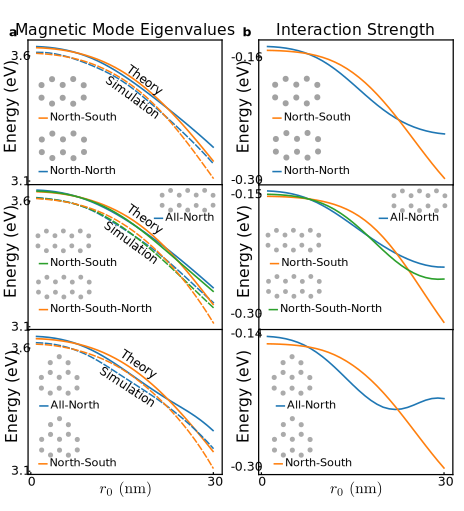
\includegraphics[width=.65\paperwidth]{magnetic_mode_eigenvalues_and_interactions.png}
\caption{Magnetic mode eigenvalues (column a), predicted and simulated, and interaction strengths (column b) for the magnetic twomer (first row), threemer chain (second row), and threemer ring (third row). All of the magnetic modes range from ~3.6 eV to ~3.1 eV. In each system, the magnetic modes exhibit multiple crossings, showing that the eigenspectrum of these magnetic systems depends on their scale. The model consistently overestimates the eigenvalues by 0.5 eV, and consistently underestimates the crossing points by less than a nanometer. The twomer has two magnetic modes, one in-phase mode (blue trace) and one out-of-phase mode (orange trace). The threemer chain has three modes, an in-phase mode (blue trace), a minimally out-of-phase mode (orange trace), and a maximally out-of-phase mode (green trace). The threemer ring exhibits three magnetic modes, but the out-of-phase modes (orange trace) are degenerate so only one is depicted. The other mode is a maximally in-phase mode (blue trace). To further emphasize the impact of scale, we have plotted the total interaction strength of each eigenmode, \textit{i.e.} the sum of each eigenvector's dot product with the electric field of all of the other dipoles. This calculation reaffirms the scale dependence and predicts mode crossings at the same scale as both the eigenvalue calculation and the simulations.}
\label{fig:magmodes}
\end{figure}

\begin{figure}
\centering
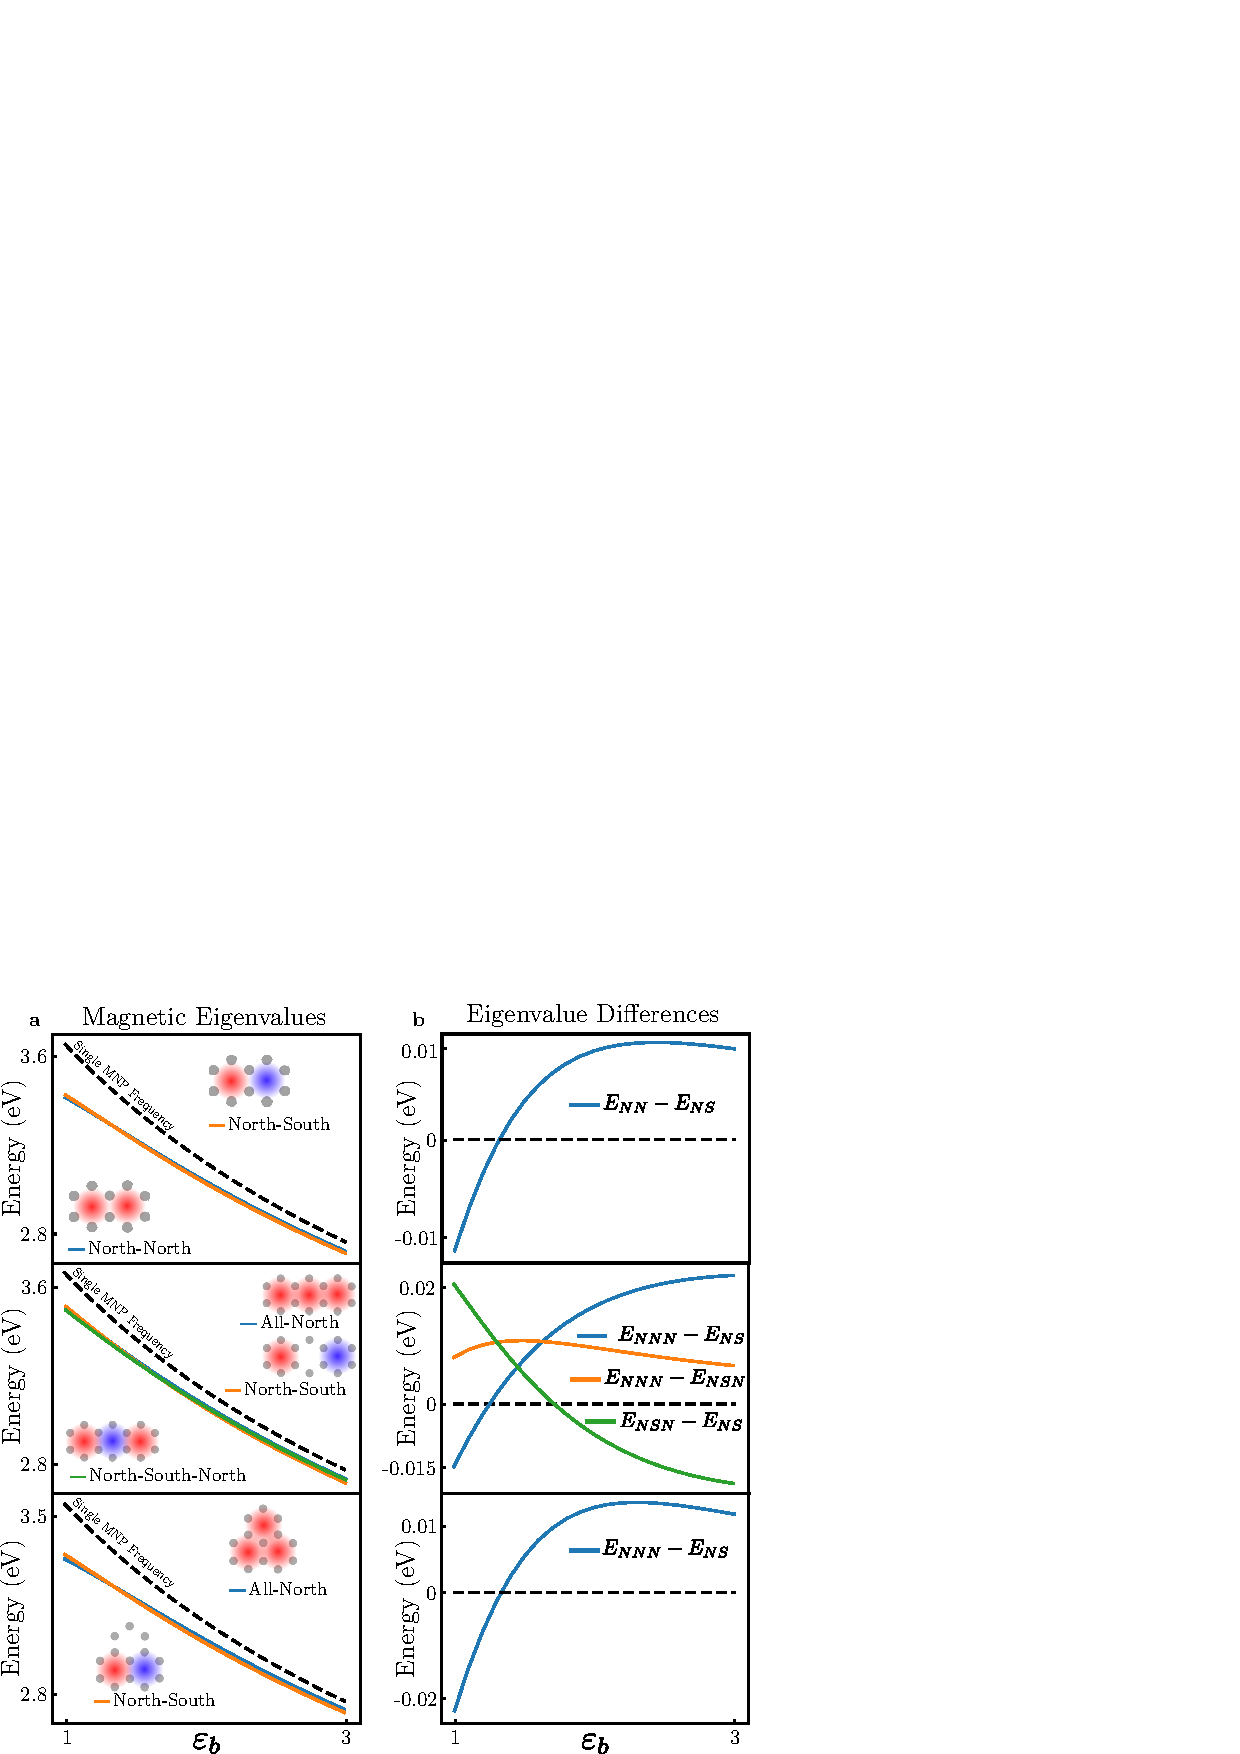
\includegraphics[width=.65\paperwidth]{dielectric_study.png}
\caption{Magnetic mode eigenvalues for twomers (first row), threemer chains (second row), and threemer rings (third row) with particle sizes of 15 nm (column a) and 30 nm (column b) as a function of the dielectric constant of an embedding medium. As the dielectric constant is increased from 1 to 3, the magnetic mode splitting decreases and the overall energy decreases. At very high dielectric values, the magnetic mode eigenvalues converge to the single particle resonance frequency. This can be explained by the increasing opacity of the medium effectively screening inter-particle interactions. It is also important to note that between $\varepsilon_b = 1$ and $\varepsilon_b = 1.5$, the magnetic modes flip order. Thus, the increasing opacity of the medium effectively decreases the scale of the system.}
\label{fig:dielectric}
\end{figure}

\begin{figure}
\centering
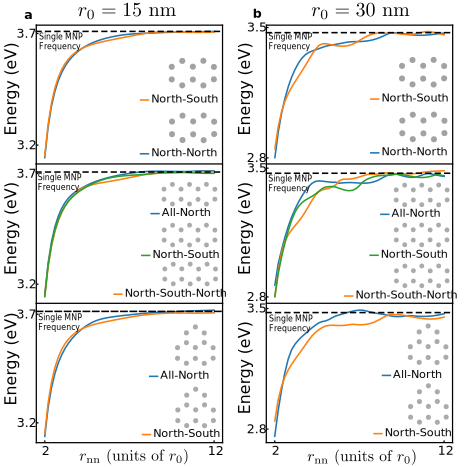
\includegraphics[width=.65\paperwidth]{spacing_study.png}
\caption{Magnetic mode eigenvalues for twomers (first row), threemer chains (second row), and threemer rings (third row) with particle sizes of 15 nm (column a) and 30 nm (column b) as a function of nearest neighbor particle spearation. The separation is plotted as a function of the particle size, in units of radii. It is important to note that as the separation distance increases, the magnetic modes cross multiple times and their eigenvalues converge to, and oscillate about the single particle frequency. This is a result of the decreasing interaction strength. In the limit of particles infinitely far away from each other, their interaction stength is zero. The oscillating nature of the eigenvalues is a result of the complex exponential dependence of the fields.}
\label{fig:spacing}
\end{figure}

\begin{figure}
\centering
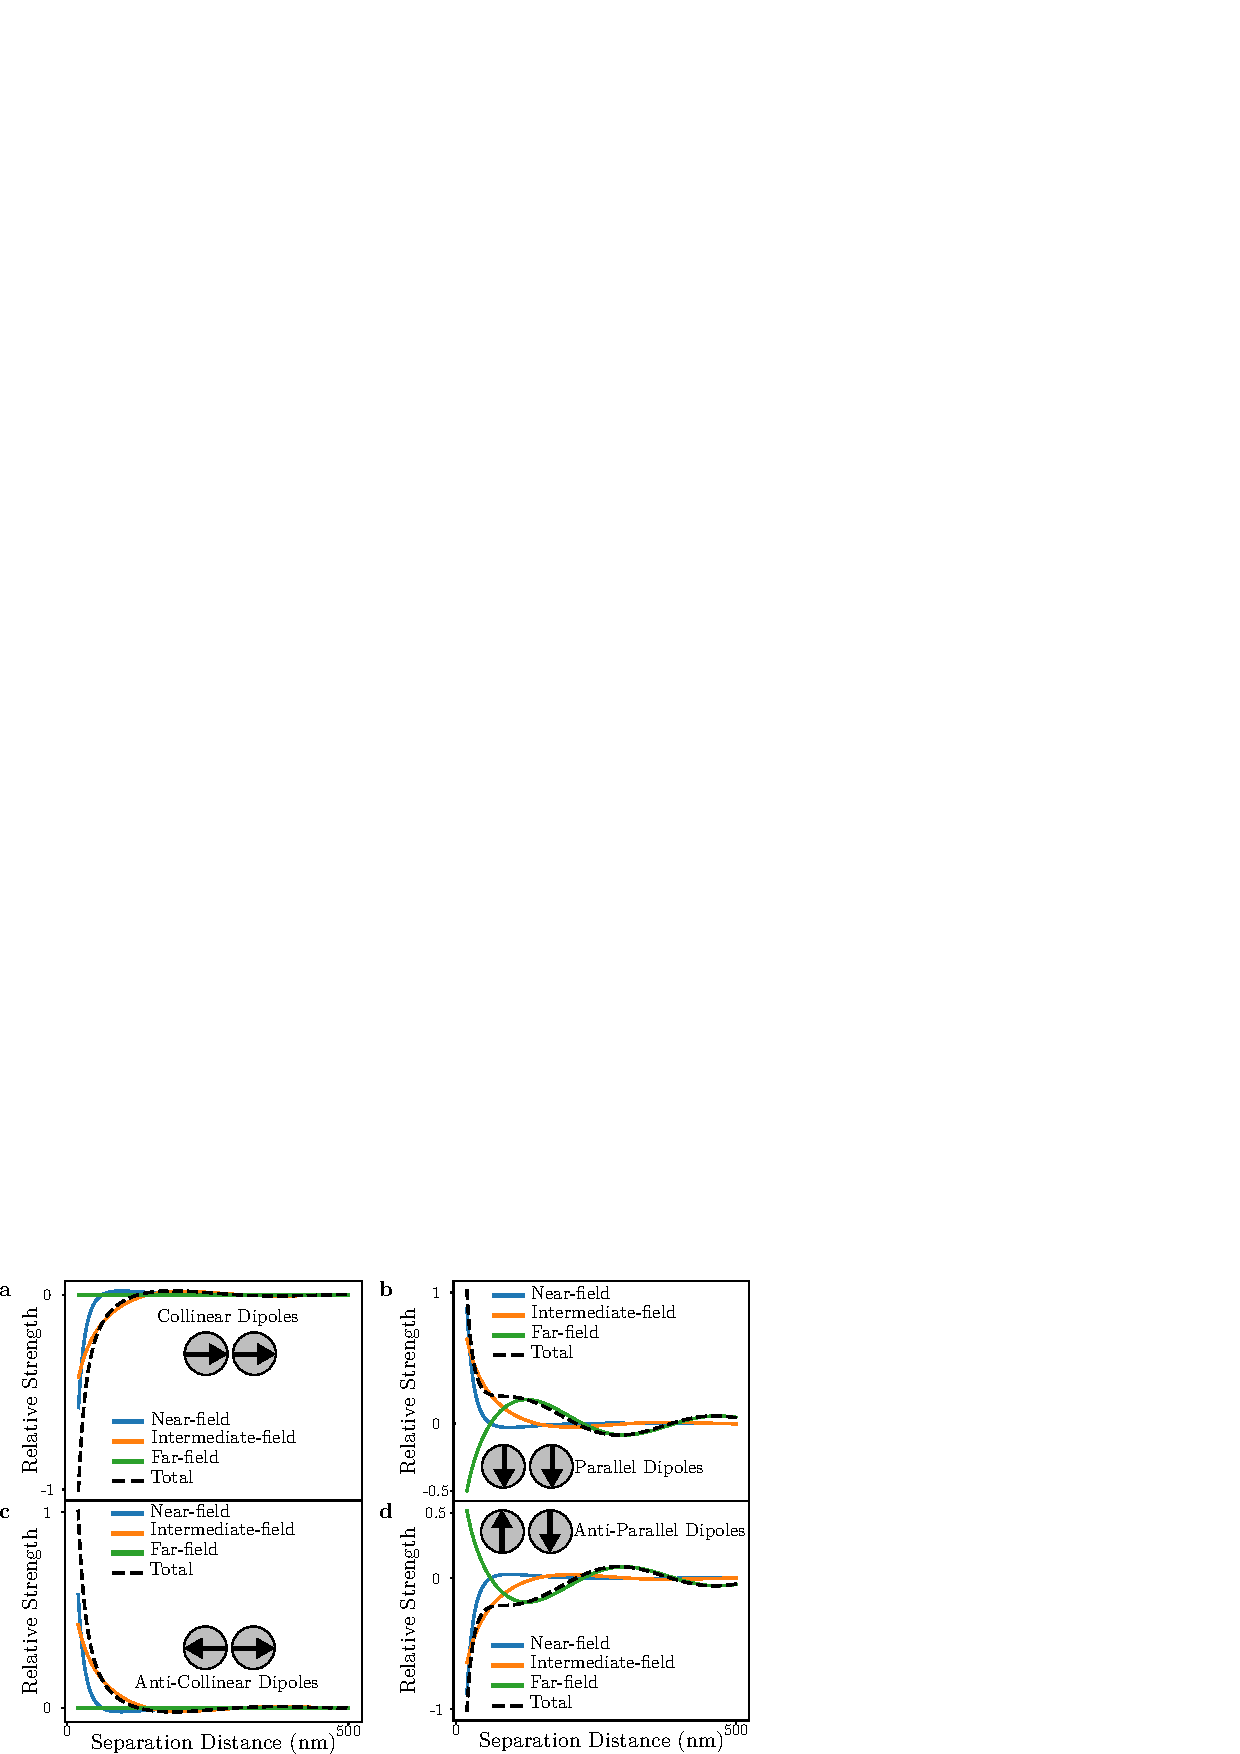
\includegraphics{dimer_interaction.png}
\caption{Relative interaction strengths for the four possible dipole arrangements of a nanoparticle dimer: collinear (a), parallel (b), anti-collinear (c), and anti-parallel (d). Plotted are the near-field (blue), intermediate-field (orange), far-field (green), and total (black, dashed) interaction strengths for each set of dipoles as a function of dipole-dipole distance. Interestingly, and stemming from the form of the dipole relay tensor, the far-field interaction term is zero for both pairs of linear dipoles. From these plots, it can be seen that the favorability of a specific dipole arrangement depends on the separation between the dipoles. This can be seen in the fact that each part of the field depends differently on the separation, and each field term contains an oscillating term. At short length scales, the interaction is dominated by the near-field. However, as the distance increases, the interaction is dominated by the intermediate-field (a and c) or the far-field (b and d). As a result, there are separation distances at which normally unfavorable arrangements become favorable. Since magnetic oligomers can be described through pairwise interactions of electric dipoles, it follows that the eigenvalues must also change order as different arrangements of electric dipoles become more and less favorable.}
\label{fig:dimers}
\end{figure}



\bibliography{references}

\end{document}
